%\begin{frame}{Opgave 4: Den adaptive metode}
%    Vi skal nu se på en anvendelse. Vi definerer en funktion ved
%\begin{align*}
%f(x) = 
%\begin{dcases}
%- \left( x - \sqrt{2} \right)^2 & x \leq \sqrt{2}\\
%\left( x - \sqrt{2} \right)^2 & x > \sqrt{2} \\
%\end{dcases}
%\end{align*} 
%    
%    Vi vil se på approksimation af integralet 
%    \begin{align}
%    \int_{0}^{3}f(x)dx    
%    \end{align}
%    % 
%\end{frame}

\begin{frame}{Approksimation af integralet}
\begin{align*}
f(x) = 
\begin{dcases}
- \left( x - \sqrt{2} \right)^2 & x \leq \sqrt{2}\\
\left( x - \sqrt{2} \right)^2 & x > \sqrt{2} \\
\end{dcases}
\end{align*} 
    
    Approksimation af integralet 
    \begin{align}
    \int_{0}^{3}f(x)dx    
    \end{align}
    % 
\end{frame}



\begin{frame}{Den adaptive metode}
    \begin{itemize}
        \item (a) Lav en Python funktion til beregning af funktionen defineret i (1).
        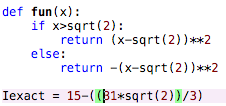
\includegraphics[]{images/1.4(a).png}
    \end{itemize}
\end{frame}


\begin{frame}{Den adaptive metode}
    \begin{itemize}
        \item (b) Vis, at den eksakte værdi af integralet er $15-\frac{31\sqrt{2}}{3}$.
        \item \begin{align*}
            \int^{\sqrt{2}}_0-(x-\sqrt{2})^2+\int^3_{\sqrt{2}}(x-\sqrt{2})^2=15-\frac{29\sqrt{2}}{3}-\frac{2^{\frac{3}{2}}}{3}=15-\frac{31\sqrt{2}}{3} 
            \end{align*} \\
            Ved at tage integralet for begge funktioner, og derefter plusse dem sammen, fås den eksakte værdi $15-\frac{31\sqrt{2}}{3}$ \\
    \end{itemize}
\end{frame}


\begin{frame}{Den adaptive metode}
    \begin{itemize}
        \item (c) Bestem integralet numerisk ved hjælp af de tre sammensatte kvadraturregler (midtpunkt, Trapez og Simpson). 
        Hvor mange ækvidistante inddelinger skal anvendes i hvert af de tre tilfælde for at opnå en fejl på mindre end $10^{-8}$?
        \item Ved Midtpunkt er fejlen mindre end $10^{-8}$ ved cirka $4096$ indelinger.\\
        Ved trapez sker dette først ved cirka $8192$, altså senere end ved midtpunkt.\\ 
        Ved Simpsonreglen sker dette ved ca $512$ og denne opnår dermed højere præcision ved færre iterationer end de foregående to.
    \end{itemize} 
\end{frame}

\begin{frame}
\begin{align*}
\begin{array}{l|c|c|c}
\text{Metode} & \text{Resultat}& \text{Fejl} &  \text{Inddelinger} \\
\hline
\text{Midtpunkt}	& 3.8645984782 \cdot 10^{-01} & 7.662 \cdot 10^{-09}	& 4096 \\
\text{Trapez}		& 3.8645985304 \cdot 10^{-01} & 2.437 \cdot 10^{-09} & 8192 \\
\text{Simpsons}		& 3.8645985931 \cdot 10^{-01} & 3.833 \cdot 10^{-09} & 512 \\
\end{array}
\end{align*}
\end{frame}

\begin{frame}{Den adaptive metode}
    \begin{itemize}
        \item (d) Lav i de tre tilfælde numeriske eksperimenter, baseret på fordobling af antal delepunkter, og brug dem til en eksperimentel bestemmelse af ordenen af de tre metoder. 
        Stemmer resultaterne med teorien? Hvis der er afvigelser, hvordan kan
        de så forklares?
        %Hvorfor springer orden så meget i Simpson efter 8192?
        \item For både trapez samt midtpunktreglen stabliseres der omkring en orden på $4$ efter et passende antal inddelinger hvilket stemmer overens med teorien, dette er dog ikke tilfældet for Simpson. Den opnår de $16$, men falder drastisk efterfølgende.
    \end{itemize}
    
$$\begin{array}{l|c|c}
\text{Metode} & \text{Inddelinger}& \text{Orden} \\
\hline
\text{Midtpunkt}	& 4		& 2 \\
\text{Trapez}		& 4		& 2 \\
\text{Simpsons}		& 16	& 4 \\
\end{array}$$
\end{frame}


\begin{frame}{Den adaptive metode}
    \begin{itemize}
        \item (e) Prøv at anvende en simpel adaptiv metode til at bestemme integralet (2). 
        Hvad sker der, hvis man inddeler i to delintervaller af samme længde. 
        Hvordan bidrager de hver til fejlen i approksimationen? 
        Angiv resultaterne for både trapezreglen og Simpsons regel.
        %Vi har svært ved at skulle dele i to delintervaller og alt det Python-fis
        \item For simpsons adaptiv: Integralet af funktionen fra $1.5$ til $3$ er præcist, idet antallet af inddelinger er ligegyldigt, da det er et tredjegradspolynomium og funktionen forbliver stabil i hele intervallet. 
        Derimod sker der fra $0$ til $1.5$ det, at funktionen skifter og der er derfor behov for et større antal inddelinger. 
        Det biddrager hermed til, at denne del af aproksimationen giver en større fejl med behov for et større antal inddelinger.
        \item For Trapez: her biddrager begge intervaller lige meget til fejlen og kræver samme antal underindelinger(512 hvis mit bud om faktor 3 er korrekt) dette skyldes at præcisionen er mindre her hvorfor approskismationen ikke er lig funktionsværdien i intervallet fra 1.5 til 3 heller.
    \end{itemize}
\end{frame}